\setcounter{secnumdepth}{1}

\chapter{Lab 4}

\begin{Task}{Question 4.1. harmonic and intermodulation distortion}
    Consider a static nonlinear system whose response is given by:\\
    \begin{equation}
        y(t) = u(t) - \frac{1}{2}u^3(t) - \frac{1}{4} u^4(t)
    \end{equation}
    At which frequencies will energy appear at the output when the input is excited by the sum of 2 sinewaves, one at frequency 4Hz and one at frequency 11Hz?    
\end{Task}

using matlab, each excited frequency has been plotted on figure \ref{fig:distortionEx}. The different amplitudes are not correct, they simply give the order of magnitude of each frequency component. A more exact simulation with the fft of the output signal is shown in figure \ref{fig:distortionExExact}.

\begin{figure}[H]
    \centering
    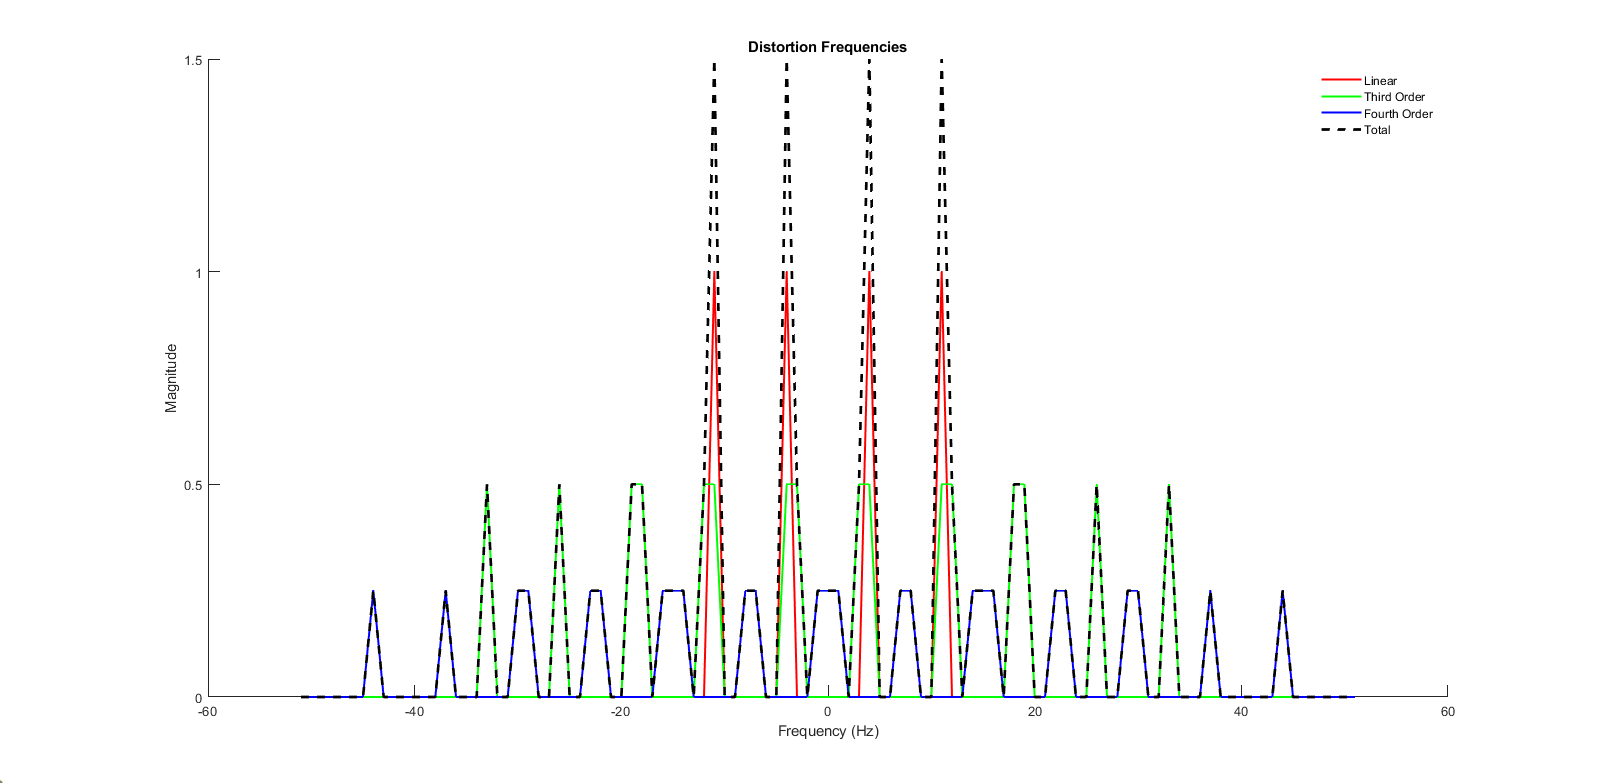
\includegraphics[width=0.8\textwidth]{part4/distortionEx.png}
    \caption{Excited frequencies - Approximation}
    \label{fig:distortionEx}
\end{figure}

\begin{figure}[H]
    \centering
    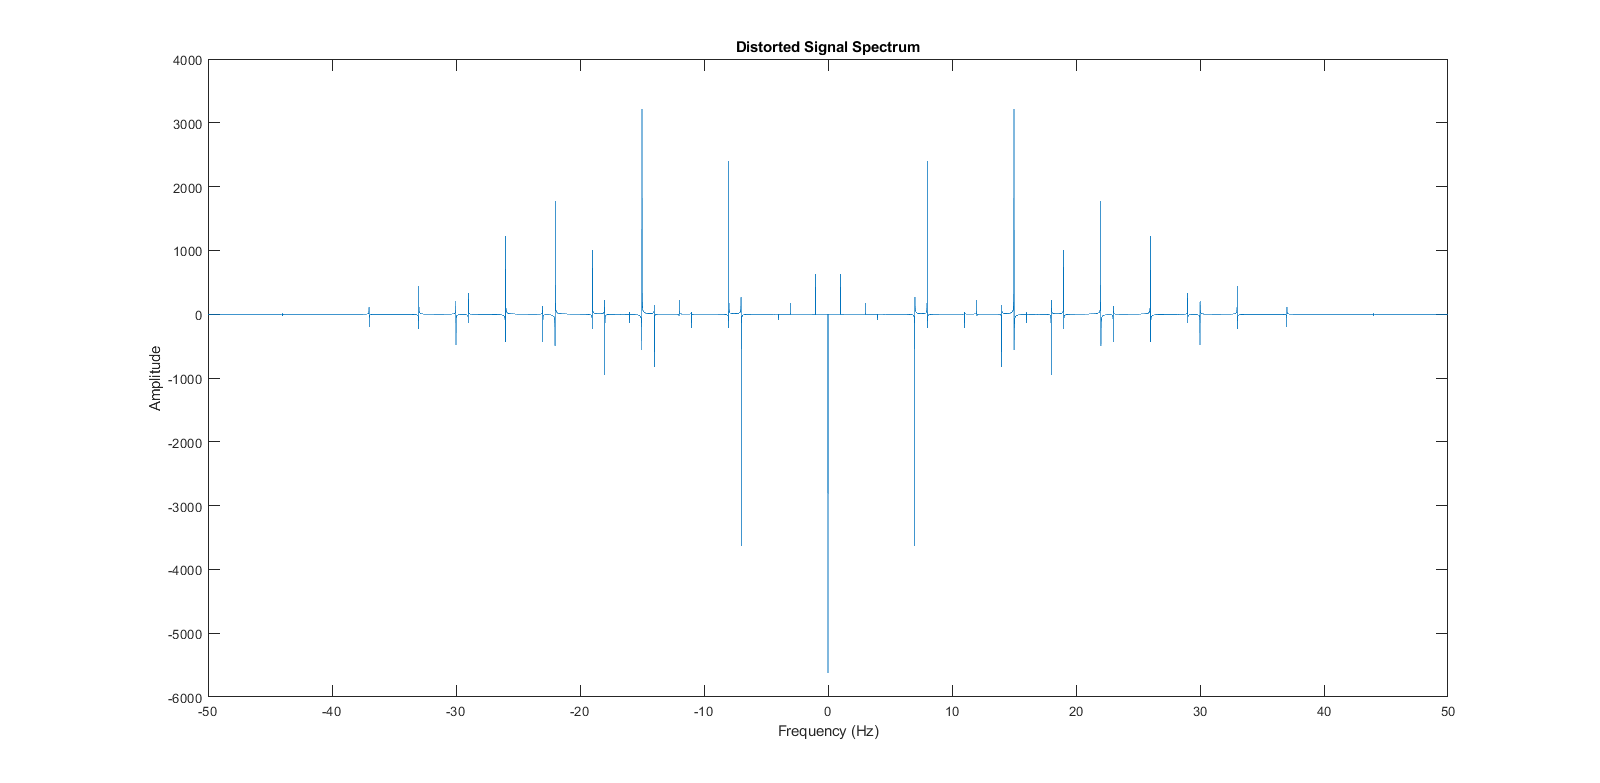
\includegraphics[width=0.8\textwidth]{part4/distortionExExact.png}
    \caption{Excited frequencies - Exact}
    \label{fig:distortionExExact}
\end{figure}

\begin{Task}{Question 4.2.}
    Design an excitation sinewave with a frequency of $100$ Hz and an amplitude of $1$ V. Plot the input signal and the output signal of the DUT in the frequency domain. What do you observe? Give a list of all possible solutions to get rid of this behaviour. Design experiments to show that the proposed solutions do indeed work.
\end{Task}

\begin{figure}[H]
    \centering
    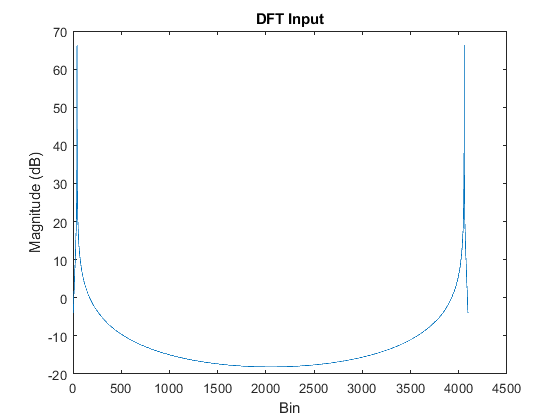
\includegraphics[width=0.8\textwidth]{part4/leakage.png}
    \caption{Initial sine wave DFT}
    \label{fig:leakage}
\end{figure}

The DFT of the sinusoidal input signal is clearly not a Dirac pulse as the chosen frequency is not at an integer bin index. \\

The size of a bin being the inverse of the signal duration $N/f_s$, we want
\begin{equation*}
    f_{\text{signal}} = k \cdot \frac{f_s}{N} \quad \text{with} \quad k \in \mathbb{N}
\end{equation*}

This is visible as there is leakage in the DFT plot. There are 3 ways of solving this:
\begin{itemize}
    \item Changing the sampling frequency $\rightarrow f_s = 9990.25 \text{Hz}$
    \item Changing the number of samples $\rightarrow N = 4100 $
    \item Changing the sine frequency $\rightarrow f_{\text{signal}} = 100.1 \text{Hz}$
\end{itemize}

\begin{figure}[H]
    \centering
    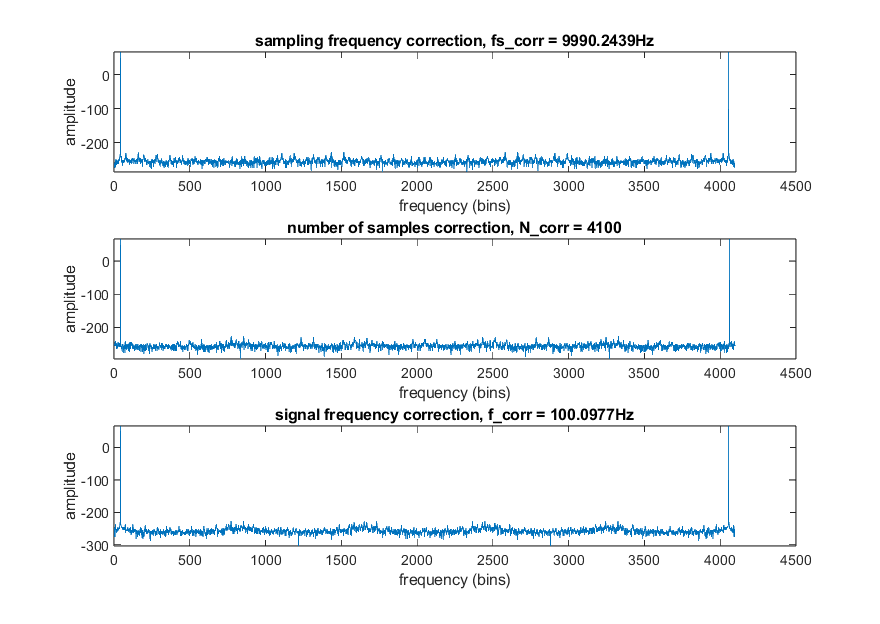
\includegraphics[width=0.8\textwidth]{part4/corrected.png}
    \caption{Corrected sine wave DFT}
    \label{fig:corrected}
\end{figure}


\begin{Task}{Question 4.3.}
    Change the excitation frequency to a frequency in the neighborhood of 100 Hz in order to solve the problem in the previous step. Use 10 different amplitudes that are spaced logarithmicaly from 100 mV to 1.1 V (logspace command in MATLAB]. Plot the DFT of the output for each amplitude. What are the frequencies at which you expect distortion to appear? Are they all present in reality? Explain.
\end{Task}

\begin{Task}{Question 4.4.}
    Plot the measurements from the previous question on an input power – output power plot. Do you see compression or expansion? From this plot, estimate the 1 dB compression or expansion point. Generate a single sine wave with the corresponding input amplitude to see how accurate your estimate is.
\end{Task}

